\cotefile{123}
\scanpage{28}
\mspage{\handwritten{\unsure{22|72}}}
% archive sheet number: 27 (inverted at the upper right)
% A single long vertical cancellation stroke runs through the typescript, from the opening paragraph into the footnote. The three enclosing deletion macros preserve this page-wide cancellation; inner deletion macros preserve the local revisions.

\deleted{un morphisme de topos $\mathrm{u}:\mathrm{E}\handwritten{\longrightarrow}\mathrm{E}'$, et ce dernier sera ``unique à isomorphisme unique près'' en termes de la donnée $\mathrm{u}^{\handwritten{*}}$ resp. $\mathrm{u}_{\handwritten{*}}$, en un sens assez clair, et qui sera d'ailleurs entièrement explicité plus bas \handwritten{(\deleted{\unsure{2|3}}3.2.1)}}

\deleted{\deleted{\unsure{2|3}}\handwritten{3}.1.2. Si $\mathrm{u}:\mathrm{E}\handwritten{\longrightarrow}\mathrm{E}'$ est un morphisme de topos, il résulte des propriétés des foncteurs adjoints \inserted{\handwritten{(I 2.11)}} que le foncteur image directe $\mathrm{u}_{\handwritten{*}}:\mathrm{E}\handwritten{\longrightarrow}\mathrm{E}'$ commute aux limites projectives, et le foncteur $\mathrm{u}^{\handwritten{*}}:\mathrm{E}'\handwritten{\longrightarrow}\mathrm{E}$ commute aux limites inductives \deleted{\unsure{(2.11)|(2.1)|(I 2.11)}}\handwritten{(${}^{*}$)}.Comme on suppose de plus que ce dernier \inserted{\handwritten{est \unsure{exact|ex.ct} à gauche i.e.}} commute aux limites projectives finies, on voit donc en particulier que $\mathrm{u}^{\handwritten{*}}$ \uline{est} \deleted{exac} \uline{exact}. \inserted{On peut donc dire que} \uline{\deleted{C}\handwritten{c}'est \deleted{donc} le foncteur image inverse} $\mathrm{u}^{\handwritten{*}}$ \deleted{qui}, dans le couple $(\mathrm{u}_{\handwritten{*}},\mathrm{u}^{\handwritten{*}})$, \uline{qui possède les propriétés d'exactitude les plus remarquables}, \deleted{assurant} Ces propriétés assurent que pour toute espèce de structure algébrique \inserted{\handwritten{$\Sigma$}}\deleted{qui peut} dont les données peuvent se décrire en termes de données de flèches entre les ensembles de base et des ensembles déduits de ceux-ci par application répétée d'opérations de limites projectives finies et de limites inductives quelconques, \inserted{\handwritten{et pour}} tout \handwritten{``}objet de $\underline{\mathrm{E}}'$ muni d'une structure d'espèce $\handwritten{\Sigma}$'' (notion qui a un sens grâce aux propriétés d'exactitude \deleted{de} internes du topos $\unsure{\mathbb{E}'|\underline{\mathrm{E}}'}$ (II 4.1)), son image \deleted{inverse} par $\mathrm{u}^{\handwritten{*}}$ est muni des mêmes structures. Plutôt que d'entrer dans la tâche peu engageante de donner un sens précis à cet énoncé et de le justifier de façon formelle, nous conseillons au lecteur de \inserted{l'expliciter et de} se convaincre de sa validité pour des espèces de structure telles que celle de groupe, d'anneau, de module sur un anneau, de comodule \deleted{ou de bimodule} sur un anneau, de bigèbre sur un anneau, de torseur sous un groupe. (Dans ces exemples, les trois premières espèces de structure se définis}
% The last word is cut at the right image edge after the visible fragment ``définis''; no unseen ending is supplied. The parenthesis is open on the source page.

% Left margin beside the body reference on L07.
\margin{\handwritten{\deleted{\unsure{(I 2.11)|(I 4.11)|(I 4.1)}}.}}

\handwritten{\figure{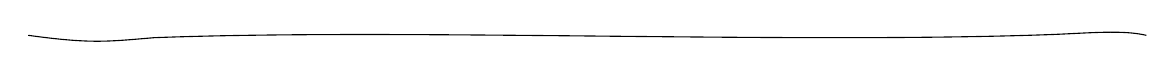
\begin{tikzpicture}[x=1cm,y=1cm]
\draw[line width=.4pt] (0,.03) .. controls (.8,-.08) and (1.0,-.05) .. (1.6,0) .. controls (4.8,.12) and (9.7,-.08) .. (13.0,.04) .. controls (13.5,.06) and (13.9,.10) .. (14.2,.03);
\end{tikzpicture}}}

\deleted{($\handwritten{*}$) \deleted{On peut} \deleted{d}\handwritten{D}'ailleurs \deleted{vérifier que}\inserted{\handwritten{(1.5 et 1.8)}}, pour un foncteur $\mathrm{u}_{\handwritten{*}}:\mathrm{E}\handwritten{\longrightarrow}\mathrm{E}'$ resp. $\mathrm{u}^{\handwritten{*}}:\mathrm{E}'\handwritten{\longrightarrow}\mathrm{E}$ donné, \deleted{\unsure{d}}\handwritten{c}e foncteur admet un adjoint à gauche (resp. à droite si et seulement si il commute aux \inserted{$\underline{\mathrm{U}}$-}limites projectives (resp. aux $\underline{\mathrm{U}}$-limites inductives). \deleted{\unsure{D'ailleurs}, c'est une conséquence immédiate de 1.2.\unsure{(ii)|(iii)|(i)}}}
% The right edge after ``droite'' is cropped; no unseen closing parenthesis has been added.
